\documentclass[]{article}
\usepackage{graphicx}
\usepackage[svgnames]{xcolor} 
\usepackage{fancyhdr}

\usepackage[hidelinks]{hyperref}
\usepackage{enumitem}
\usepackage[many]{tcolorbox}
\usepackage{listings }
\usepackage[a4paper, total={6in, 8in}]{geometry}
\usepackage{afterpage}
\usepackage{amssymb}
\usepackage{caption}
\usepackage{pdflscape}
\usepackage{textcomp}
\usepackage{xecolor}
\usepackage{rotating}
\usepackage[Kashida]{xepersian}
\usepackage[T1]{fontenc}
\usepackage{tikz}
\usepackage[utf8]{inputenc}
\usepackage{PTSerif} 
\usepackage{seqsplit}
\usepackage{changepage}



\usepackage{listings}
\usepackage{xcolor}
\usepackage{sectsty}
 
\definecolor{codegreen}{rgb}{0,0.6,0}
\definecolor{codegray}{rgb}{0.5,0.5,0.5}
\definecolor{codepurple}{rgb}{0.58,0,0.82}
\definecolor{backcolour}{rgb}{0.95,0.95,0.92}
 
\NewDocumentCommand{\codeword}{v}{
\texttt{\textcolor{blue}{#1}}
}
\lstset{language=java,keywordstyle={\bfseries \color{blue}}}

\lstdefinestyle{mystyle}{
    backgroundcolor=\color{backcolour},   
    commentstyle=\color{codegreen},
    keywordstyle=\color{magenta},
    numberstyle=\tiny\color{codegray},
    stringstyle=\color{codepurple},
    basicstyle=\ttfamily\normalsize,
    breakatwhitespace=false,         
    breaklines=true,                 
    captionpos=b,                    
    keepspaces=true,                 
    numbers=left,                    
    numbersep=5pt,                  
    showspaces=false,                
    showstringspaces=false,
    showtabs=false,                  
    tabsize=2
}

\lstset{style=mystyle}

 \settextfont[BoldFont={XB Zar bold.ttf}]{XB Zar.ttf}


\setlatintextfont[Scale=1.0,
 BoldFont={LiberationSerif-Bold.ttf}, 
 ItalicFont={LiberationSerif-Italic.ttf}]{LiberationSerif-Regular.ttf}





\newcommand{\inputsample}[1]{
    ~\\
    \textbf{ورودی نمونه}
    ~\\
    \begin{tcolorbox}[breakable,boxrule=0pt]
        \begin{latin}
            \large{
                #1
            }
        \end{latin}
    \end{tcolorbox}
}

\newcommand{\outputsample}[1]{
    ~\\
    \textbf{خروجی نمونه}

    \begin{tcolorbox}[breakable,boxrule=0pt]
        \begin{latin}
            \large{
                #1
            }
        \end{latin}
    \end{tcolorbox}
}

\newenvironment{changemargin}[2]{%
\begin{list}{}{%
\setlength{\topsep}{0pt}%
\setlength{\leftmargin}{#1}%
\setlength{\rightmargin}{#2}%
\setlength{\listparindent}{\parindent}%
\setlength{\itemindent}{\parindent}%
\setlength{\parsep}{\parskip}%
}%
\item[]}{\end{list}}


\definecolor{foldercolor}{RGB}{124,166,198}
\definecolor{sectionColor}{HTML}{ff5e0e}
\definecolor{subsectionColor}{HTML}{008575}

\definecolor{listColor}{HTML}{00d3b9}

\definecolor{umlrelcolor}{HTML}{3c78d8}


\defpersianfont\titr[Scale=1.5]{Lalezar-Regular.ttf}

\defpersianfont\fehrest[Scale=1.2]{Lalezar-Regular.ttf}

\sectionfont{\color{sectionColor}}  % sets colour of sections



\subsectionfont{\color{subsectionColor}}  % sets colour of sections

\renewcommand{\labelitemii}{$\circ$}


\renewcommand{\baselinestretch}{1.1}
\setlength{\parskip}{1.2pt}


\begin{document}


%%% title pages
\begin{titlepage}
\begin{center}

\textbf{ \Huge{به نام خدا} }
        
\vspace{0.2cm}


\includegraphics[width=0.4\textwidth]{sharif1.png}\\
\vspace{0.2cm}
\textbf{ \Huge{\emph درس برنامه‌سازی پیشرفته} }\\
\vspace{0.25cm}
\textbf{ \Large{آموزش UML} }
\vspace{0.2cm}
       
 
      \large \textbf{دانشکده مهندسی کامپیوتر}\\\vspace{0.1cm}
    \large   دانشگاه صنعتی شریف\\\vspace{0.2cm}
       \large   ﻧﯿﻢ سال دوم 99-98 \\\vspace{0.10cm}
      \noindent\rule[1ex]{\linewidth}{1pt}
اساتید:\\
    \textbf{{مهدی مصطفی‌زاده، ایمان عیسی‌زاده، امیر ملک‌زاده، علی چکاه}}



   

        \vspace{0.10cm}
نگارش و تهیه محتوا:\\
    \textbf{{زهرا یوسفی جمارانی}}
    

       \vspace{0.10cm}
       تنظیم داک:\\
    \textbf{{امیرمهدی نامجو}}
    
        \vspace{0.05cm}

\end{center}
\end{titlepage}
%%% title pages


%%% header of pages
\newpage
\pagestyle{fancy}
\fancyhf{}
\fancyfoot{}
\cfoot{\thepage}
\lhead{آموزش UML}
\rhead{
\includegraphics[width=0.1\textwidth]{sharif.png}\\
دانشکده مهندسی کامپیوتر
}
\chead{پروژه برنامه‌سازی پیشرفته}
%%% header of pages
\renewcommand{\headrulewidth}{2pt}

\KashidaOff


 \Large \textbf{\\
}


\section*{{\titr مقدمه - UML چیست؟}}

\lr{Unified Modeling Language} یک زبان مدلسازی در مهندسی نرم افزار است که هدف اصلی آن تعریف یک روش استاندارد برای نمایش طراحی سیستم هاست.این زبان در ابتدا در سال های  \lr{1994-95} توسعه یافت و امروزه به صورت گسترده برای مدلسازی استفاده میشود.

\begin{center}


\includegraphics[width=0.22\textwidth]{images/image4.png}

\end{center}



\section*{{\titr چرا UML ?}}

برای شروع یک پروژه ممکن است فردی بدون هیچ فکر قبلی درباره ابعاد پروژه شروع به کد زدن کند و سپس به مرور کد ها را اضافه کند؛ مشکل این روش آن است که در نهایت این پروژه یک معماری مناسب نخواهد داشت و شاید حتی در میانه کار کدنویس گیج شود!

 بهترین کار برای جلوگیری از این مشکل داشتن یک نگاه اجمالی بر پروژه  و در نظر گرفتن همه ی ابعاد پروژه است؛ این کار با مدلسازی کل پروژه قبل از شروع به کد زدن توسط زبان‌های مدلسازی از جمله \lr{UML} انجام می‌شود.
 
در نتیجه استفاده از یو ام ال هزینه تغییر شیوه ی معماری و تعویض کد را به شدت کاهش می‌دهد!

در ابتدا شاید کشیدن \lr{UML} کمی سخت باشد اما با توجه به اینکه چیزی که شما می‌کشید مبنای شروع کد زنی شما برای فاز اول پروژه خواهد بود، لازم است تا با تسلط تمام کشیده شود؛پس از پاک کردن و از اول شروع کردن در مرحله \lr{UML} نترسید! 

نمودارهای کلاس (\lr{class diagram}) مشهور ترین نمودارهای \lr{UML} هستند که در اینجا به توضیح آن می‌پردازیم.

\newpage

\section*{{\titr اصول و قواعد }}

نکاتی که باید در طراحی نمودارهای خود به آن ها توجه کنید:

\begin{itemize}

\item
نام کلاس‌های شما باید معنا دار باشد

\item
تمام فرآیندها، مسیرها و روابط باید مشخص شود

\item
متودها و صفات هر کلاس باید مشخص شود



\end{itemize}


\subsection*{{\titr عناصر مهم در نمودار کلاس:}}

\begin{enumerate}

\item

نام کلاس

\item
صفات

\item
اعمال

\item
روابط

\end{enumerate}


\begin{center}

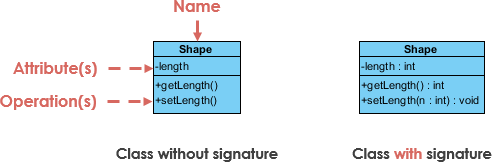
\includegraphics[width=0.85\textwidth]{images/image11.png}

\end{center}

\begin{itemize}[label=\textcolor{listColor}{$\blacklozenge$}]
  \item
   {\fehrest \textcolor{listColor}{نام کلاس:}}
   

   \begin{enumerate}

\item
   با حرف بزرگ شروع شود
   
\item
پررنگ نوشته شود

\item
در وسط نوشته شود (تراز در وسط)

\item
اگر کلاس \lr{abstract} است به صورت \textit{\lr{italic}} نوشته شود

   
   
   
   \end{enumerate}
  
  \newpage
  
  \item
   {\fehrest \textcolor{listColor}{صفات: }}

   
   در این بخش باید صفاتی که این کلاس مدل می‌کند را اضافه کنید مثلا برای یک دانشجو می‌توان مدلسازی زیر را قائل شد:
   
   
  \begin{center}

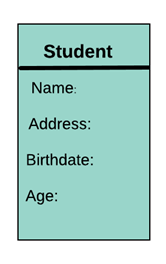
\includegraphics[]{images/image15.png}

\end{center}

باید برای هر صفت دسترسی آن نیز مشخص شود که به صورت زیر است:

\begin{itemize}[label={\textbullet}]

\item
\lr{Public} (دسترسی در همه جا):    +

\item
\lr{Private} (دسترسی درون کلاسی) :    -

\item
\lr{Protected} (دسترسی در کلاس های فرزند) :    \#

\item
\lr{Package} (درون پکیج) :    \char`~



\end{itemize}

نکات:

\begin{itemize}[label={\textbullet}]

\item
صفات باید نام مناسب داشته باشند.

\item
برای صفات باید نوع داده آن‌ها را مشخص کنید؛ مثلا: \lr{String} ،\lr{int} و …..


\end{itemize}
   
   \item
   {\fehrest \textcolor{listColor}{اعمال :}}
   
   
   در این قسمت باید تابع های هر کلاس  را اضافه کنید و باید توجه داشته باشید که:
   
\begin{itemize}[label={\textbullet}]

\item
ابتدا باید نوع دسترسی تابع را مشخص کنید

\item
نام معناداری انتخاب کنید

\item
پارامتر‌های ورودی را همراه نوع داده‌ی آن مشخص کنید

\item
نوع داده‌ای که تابع بر می‌گرداند \lr{(return type)} را  در انتهای خط پس از \linebreak علامت : مشخص کنید

مثلا :

\begin{center}
\begin{latin}
+ method ( param : int ) : String

\end{latin}
\end{center}



\end{itemize}   


\begin{center}


\begin{figure}[h!]

  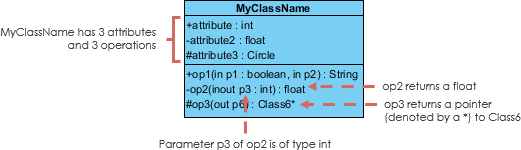
\includegraphics[width=1.0\textwidth]{images/image7.png}
  \captionsetup{labelformat=empty}
  \caption{به \lr{in}  و \lr{inout}  در شکل توجه نکنید
}
\end{figure}


\end{center}  
\newpage

 
 \item
   {\fehrest \textcolor{listColor}{روابط: }}
  
  \begin{itemize}[label={\textbullet}] 
  \item
  
  وابستگی
  
  \item
تعمیم و وراثت

\item

انجمنی

\item

تفهیم

\end{itemize}
   
    \begin{center}

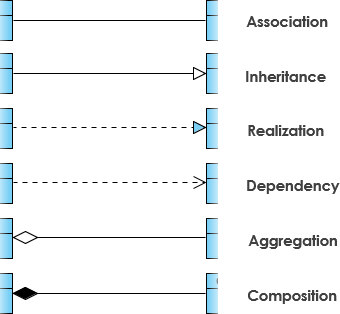
\includegraphics[]{images/image2.png}

\end{center}
\newpage
\begin{itemize}[label=\textcolor{umlrelcolor}{$\blacksquare$}]
 \item
   {\fehrest \textcolor{umlrelcolor}{وابستگی :(Dependency)
 }}
 

 
 وابستگی به معنای رابطه بین دو یا تعداد بیشتری کلاس است که ممکن است تغییر در یک کلاس، تغییر در کلاس دیگر را ایجاب کند.
 
همان طور که از اسم این رابطه مشخص است به این معناست که یک کلاس به دیگری وابسته است.


   \begin{center}

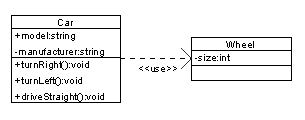
\includegraphics[]{images/image3.png}

\end{center}


 \item
   {\fehrest \textcolor{umlrelcolor}{تعمیم و وراثت ( Inheritance and Generalization ):
 }}
 

 
 این رابطه کلاس فرزند را به پدر مربوط می کند؛ در واقع کلاس فرزند از پدر ارث بری می‌کند.
توجه کنید ازین رابطه برای interface  ها نباید استفاده کرد!!!


   \begin{center}

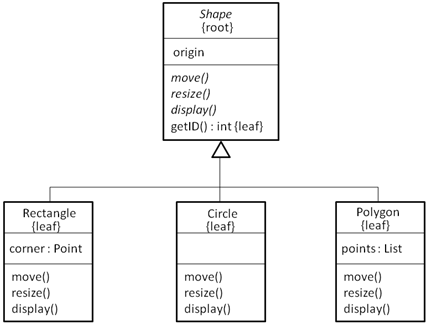
\includegraphics[width=0.75\textwidth]{images/image10.png}

\end{center}

\newpage

 \item
   {\fehrest \textcolor{umlrelcolor}{انجمنی  :(Association)
 }}


 
 برای نمایش روابط ایستا بکار می‌رود مثلا:  کارمند \underline{کار می‌کند} برای کارخانه و یا:
 
 

    \begin{center}

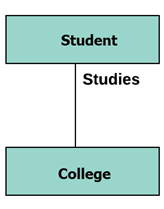
\includegraphics[]{images/image5.png}

\end{center}
 
 انواع روابط انجمنی: 
 
 \begin{enumerate}

\item
تجمع (\lr{Aggregation}):
 
 این رابطه یک نوع خاص از روابط انجمنی است که رابطه بین کل و اجزای آن را مدل می‌کند. توجه کنید در این رابطه کلاس ها به طور کامل به هم وابسته نیستند؛ مثلا 
در رابطه‌ی زیر کلاس دانشگاه حتی اگر دانشجو نیز نباشد باقی خواهد ماند.

\begin{center}


  
\includegraphics[]{images/image9.png}
 



\end{center} 
 
 \newpage
 \item
ترکیب (\lr{Composition}):
 
این رابطه نوع قوی‌تر رابطه‌ی قبلی است به این صورت که دو یا چند کلاس کاملا به هم وابسته‌اند؛ مثلا:


\begin{center}


  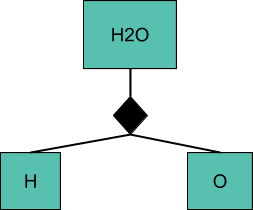
\includegraphics[]{images/image13.png}
 



\end{center}  

در اینجا اگر \lr{O} یا \lr{H} نباشد کلاس \lr{H2O} نمی‌تواند باشد.



\item
نرمال (\lr{Normal}):
 
 رابطه‌ی عادی بین دو کلاس مثلا:
 
 
 \begin{center}


  
\includegraphics[]{images/image6.png}
 



\end{center}  
 
 
\end{enumerate}
 
 \newpage
 
  \item
   {\fehrest \textcolor{umlrelcolor}{تفهیم   :(Realization)
 }}
 

 
 این رابطه به نام تفهیم یا تحقق نام دارد و کلاس های دیگر وظیفه‌ی تکمیل کردن دارند؛ مثلا برای interface  و enum  ها بکار می‌رود.



 \begin{center}


  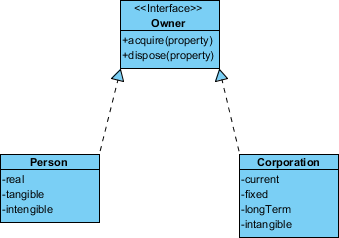
\includegraphics[width=0.75\textwidth]{images/image12.png}
 



\end{center}

 
\end{itemize}


 \item
   {\fehrest \textcolor{listColor}{نکات: }}
   
   \begin{enumerate}

\item
برای نمایش \lr{static}  از زیر خط (\lr{underline}) استفاده می‌کنیم.   
\item
چندی (Multiplicity) را نیز می‌توانید با نوشتن عدد یک (نمایندهٔ یک نمونه) و یا $*$ (نمایندهٔ چند نمونه) روی خط رابطه نمایش دهید. (مانند نمونه)   
 
   \end{enumerate}
   
   \newpage
    \item
   {\fehrest \textcolor{listColor}{نمونه: }}
   

	 \begin{center}


  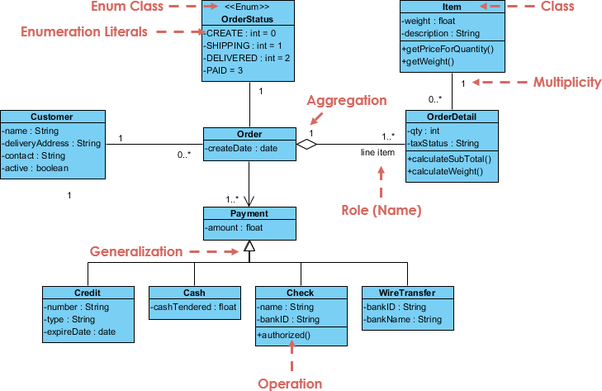
\includegraphics[width=1.0\textwidth]{images/image14.png}
 



\end{center}


\end{itemize}






\newpage

\section*{{\titr نرم افزارها و سایت های رسم UML}}

\begin{enumerate}

\item

\href{https://www.lucidchart.com/pages/}{\textcolor{blue}{\underline{سایت Lucidchart}}} 


\item

\href{https://products.office.com/en/visio/flowchart-software}{\textcolor{blue}{\underline{نرم افزار \lr{Microsoft Visio}}}} 


\item

\href{https://www.umlet.com/changes.htm}{\textcolor{blue}{\underline{نرم افزار UMLet}}} 


\item

\href{https://online.visual-paradigm.com/}{\textcolor{blue}{\underline{نرم افزار \lr{Visual Paradigm}}}} 


\item

\href{https://www.modelio.org/}{\textcolor{blue}{\underline{نرم افزار Modelio}}} 


\item

\href{https://app.diagrams.net/}{\textcolor{blue}{\underline{سایت \lr{Draw.io}}}} 



\end{enumerate}


\end{document}









